\section{Small-amplitude surface waves (73-84)}

\begin{figure}[!h]
    \centering
    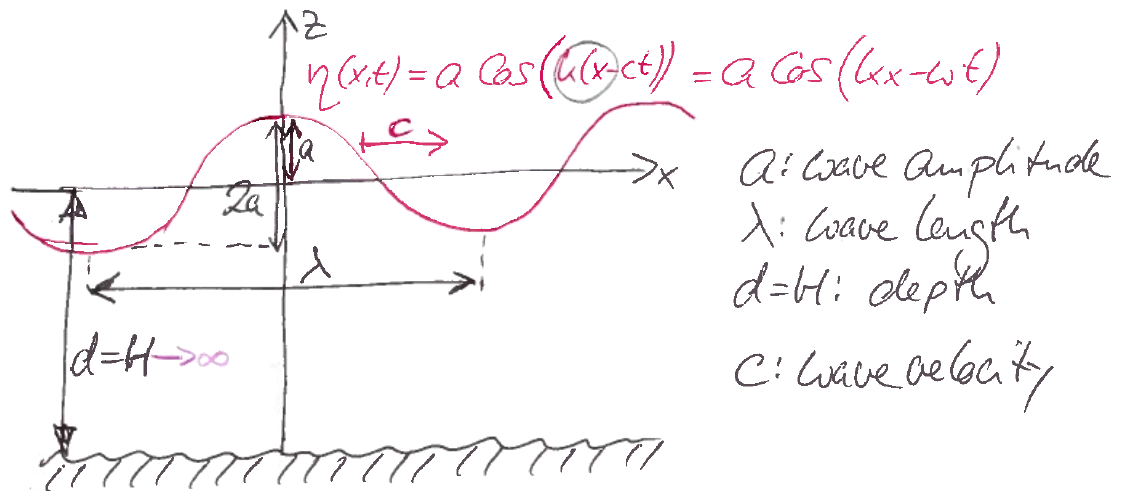
\includegraphics[width=.9\textwidth]{week6/surface-waves}\\
    \caption{}
    \label{fig:surface-waves}
\end{figure}

\fref{fig:surface-waves} shows a surface wave. Here $k$ is the wave number, $\tau$ the oscillation period, and $\omega$ the circular frequency.

\begin{align}
k &= \frac{2\pi}{\lambda}\\
\omega &= \frac{2\pi}{\tau} = 2\pi f\\
c &= \frac{\lambda}{\tau} = \lambda f = \frac{\omega}{k}
\end{align}

\textbf{Questions}:
\begin{enumerate}
\item how does $c$ depend on $\lambda$, $d$, $a$, ...
\item how does the fluid particles (below the surface) move?
\item pathlines? expectation: more fluid motion close to the surface than in great depth.
\end{enumerate}

\textbf{Assumptions}:
Incompressibility:
\begin{equation}
\rho=\rho_0\ ,\quad \vec{\nabla}\cdot\vec{u}=0
\end{equation}

No friciton. Euler equation:
\begin{equation}
\rho_0\left(\pdiff{\vec{u}}{t}+\left(\vec{u}\cdot\vec{\nabla}\right)\vec{u}\right) = \vec{f}\mathrm{ext}-\vec{\nabla}p
\end{equation}

Gravitational force density:
\begin{equation}
\vec{f}_\mathrm{ext} = -\rho_0g\vec{e}_z = -\vec{\nabla}(\rho_0 gz)
\end{equation}

small amplitude waves:
\begin{equation}
a\ll \lambda,d
\end{equation}

deep water waves:
\begin{equation}
\lambda\ll d
\end{equation}

\begin{equation}
a\ll\lambda\ll d
\end{equation}

\begin{equation}
\biggm\vert\pdiff{\vec{u}}{t}\biggm\vert \approx \frac{\Delta u}{\Delta t} \approx \frac{u-0}{\tau/4} \approx \frac{u}{\tau} \approx \frac{a}{\tau^2}
\end{equation}

\begin{align}
|(\vec{u}\cdot\vec{\nabla})\vec{u}| &\approx u\frac{\Delta u}{\Delta x}\\
&\approx u\frac{u}{\lambda}=\frac{u^2}{\lambda} = \frac{1}{\lambda}\frac{a^2}{\tau^2}
\end{align}

\begin{align}
\frac{|(\vec{u}\cdot\vec{\nabla})\vec{u}|}{|\partial \vec{u}/\partial t|} \approx \frac{\frac{1}{\lambda}\frac{a^2}{\tau^2}}{\frac{a}{\tau^2}} = \frac{a}{\lambda} \ll 1
\end{align}

"Surviving" part of the Euler equation:
\begin{equation}
\pdiff{\vec{u}}{t}=-\vec{\nabla}\left(gz+\frac{p}{\rho_0}\right)
\end{equation}

we do the curl
\begin{equation}
\vec{\nabla}\times\pdiff{\vec{u}}{t}=-\vec{\nabla}\times\vec{\nabla}\left(gz+\frac{p}{\rho_0}\right) = 0
\end{equation}

\begin{equation}
\vec{\nabla}\times\vec{u}=\mathrm{constant}\require0
\end{equation}
This constant has to be the same everywhere:
\begin{equation}
\mathrm{constant}(z=0) = \mathrm{constant}(z=-\infty)=0
\end{equation}

\begin{equation}
\vec{u}=\vec{\nabla}\Phi
\end{equation}

with incompressibility
\begin{equation}
0=\vec{\nabla}\vec{u}=\vec{\nabla}\cdot\vec{\nabla}\Phi=\left(\ppdiff{}{x}+\ppdiff{}{z}\right)\Phi(x,z,t)
\end{equation}

\textbf{Question:} how shall we solve this linear differential equation? 

We solve it via factorization:
\begin{equation}
\Phi(x,z,t)=X(x)Z(z)T(t)
\end{equation}

\begin{align}
\begin{split}
\frac{1}{X(x)Z(z)T(t)}  \left[ \ppdiff{}{x}(X(x)Z(z)T(t)) + \ppdiff{}{z}(X(x)Z(z)T(t))\right] &=  \frac{1}{X(x)}\ppdiff{X(x)}{x} \\
&\hspace{5mm}+\frac{1}{Z(z)}\ppdiff{Z(z)}{z}
\end{split} \\
&= 0
\end{align}

\begin{equation}
\frac{1}{X(x)}\ppdiff{X(x)}{x} = \mathrm{constant} = \frac{1}{Z(z)}\ppdiff{Z(z)}{z}
\end{equation}

\begin{align}
\ppdiff{X(x)}{x}+k^2X(x) &= 0 \\
\ppdiff{Z(z)}{z}+k^2Z(z) &= 0 
\end{align}

\begin{align}
X(x) &= e^{\pm ikx} \\
Z(z) &= e^{\pm kz}
\end{align}

\begin{equation}
\Phi(x,z,t) = Ae^{\pm ikx}e^{\pm kz} T(t)
\end{equation}

\subsection{First boundary condition}
$(z=-d=-\infty)$

\begin{align}
\vec{u}|_{z=-\infty} &= 0
\leadsto
\Phi(z=-\infty)&=\mathrm{constant} =0\\
\leadsto
\Phi(x,z,t) = f_+(x,t)e^{kz}+f_-(x,t)e^{-kz}
\end{align}

\begin{equation}\label{eq:surface-phi}
\Phi(x,c,t) = A e^{\pm ikx} e^{kz} T(t)
\end{equation}

\subsection{Second boundary condition}(surface)
\begin{equation}
p(x,z,t)|_{z=\eta(x,t)} = p_0
\end{equation}

\begin{align}
\pdiff{\vec{u}}{t} &= \pdiff{}{t}\left(\vec{\nabla}\Phi\right) = -\vec{\nabla}\left(gz+\frac{p}{\rho_0}\right) \\
\leadsto
\vec{\nabla}\left(\pdiff{\Phi}{t}+gz+\frac{p}{\rho_0}\right)&=0
\end{align}

\begin{align}
\left(\pdiff{\Phi}{t}+gz+\frac{p}{\rho_0}\right)\biggm\vert_{z=\eta(x,t)} = \left(\pdiff{\Phi}{t}+gz\right) + \frac{p_0}{\rho_0} = \mathrm{constant}
\end{align}

Gauge transformation:
\begin{equation}
\Phi \rightarrow \Phi + \left(\mathrm{constant}-\frac{p_0}{\rho_0}\right)t
\end{equation}
We are allowed to do this because the velocity field $\vec{u}=\vec{\nabla}\Phi$ does not change with this transformation.

\begin{align}
\left(\pdiff{\Phi}{t}+gz\right)\biggm\vert_{z=\eta(x,t)}&=0\\
\pdiff{\Phi}{t}\biggm\vert_{z=\eta(x,t)} &= -g\eta(x,t)\label{eq:surface-phi-eta}
\end{align}

If we want to determine $\Phi$ i.e. $T(t)$ we need another equation relating $\Phi$ and $\eta$, so that we get rid of $\eta$. This is the kinematic boundary condition.

\newpage
\subsection{Kinematic boundary condition}

\begin{figure}[!h]
    \centering
    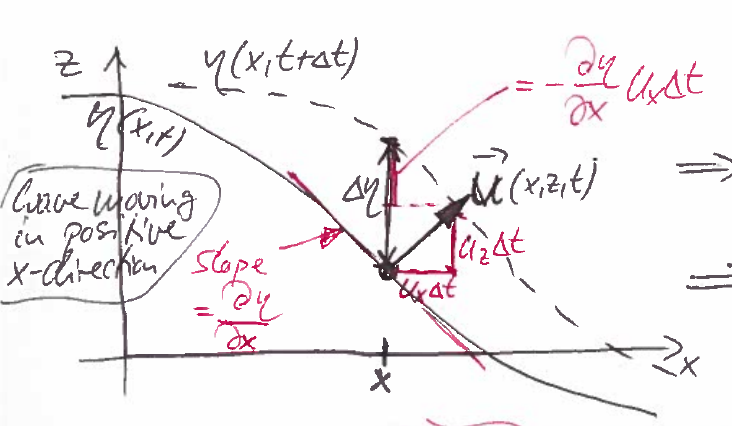
\includegraphics[width=.9\textwidth]{week6/kinematic-boundary}\\
    \caption{}
    \label{fig:kinematic-boundary}
\end{figure}

\begin{align}
\Delta \eta &= u_z\Delta t-\pdiff{\eta}{x}u_x\Delta t\\
\leadsto
\pdiff{\eta}{t}&\approx\frac{\Delta \eta}{\Delta t}\\
&= u_z-\pdiff{\eta}{x}u_x\\
&\approx u_z
\end{align}

\begin{align}
\pdiff{\Phi}{x}\biggm\vert_{z=\eta} &= u_z\biggm\vert_{z=\eta(x,t)} = \pdiff{\eta(x,t)}{t} \\
&= \pdiff{}{t}\left(\frac{(-1)}{g}\pdiff{\Phi}{t}\biggm\vert_{z=\eta}\right) \\
&= -\frac{1}{g}\ppdiff{\Phi}{t}\biggm\vert_{z=\eta}
\end{align}

again $a\ll \lambda$
\begin{equation}
\pdiff{\Phi}{z}\biggm\vert_{z\approx0} + \frac{1}{g}\ppdiff{\Phi}{t}\biggm\vert_{z\approx0}=0
\end{equation}
Now we can determine $T(t)$ by inserting the expression for $\Phi$ in \eqref{eq:surface-phi}.

\begin{align}
\pdiff{\Phi}{z}\biggm\vert_{z=0} &= Ae^{\pm ikx}ke^{kz}T(t)\biggm\vert_{z=0}\\
&= Ae^{\pm ikx} T(t)\\
&\require -\frac{1}{g} \ppdiff{\Phi}{t}\biggm\vert_{z=0} = -\frac{1}{g}Ae^{\pm ikx}\ppdiff{T(t)}{t}
\end{align}

\begin{equation}
\ppdiff{T(t)}{t}+gkT(t)=0
\end{equation}

\begin{equation}
T(t)e^{\pm i\sqrt{gk}t} = e^{\pm i\omega t}
\end{equation}

\begin{equation}
\Phi(x,z,t)=Ae^{kz}e^{\pm ikx}e^{\pm i\omega t}
\end{equation}
Using Euler relations this can be rewritten as
\begin{equation}
\Phi(x,z,t)=Ae^{kz}\sin(kx-\omega t)
\end{equation}
From this expression for the velocity potential we can calculate the surface function $\eta(x,t)$ via the relation \eqref{eq:surface-phi-eta}:

\begin{align}
\eta(x,t) &= \frac{(-1)}{g}\pdiff{\Phi}{t}\biggm\vert_{z=\eta(x,t)}\\
&= \frac{(-1)}{g}A(-\omega)\cos(kx-\omega t)e^{kz}\biggm\vert_{z=\eta}\\
&= \frac{\omega}{g}A\cos(kx-\omega t)e^{k\eta(x,t)}\\
&=\frac{\omega}{g}A\cos(kx-\omega t)
\end{align}
This is the expression as in \fref{fig:surface-waves}. The wave velocity is given by
\begin{equation}
c = \frac{\omega}{k} = \frac{\sqrt{gk}}{k} = \sqrt{\frac{g}{k}} = \sqrt{\frac{g\lambda}{2\pi}}
\end{equation}
Surface waves with a large wave length propagate faster than those with a short wave length.

\textbf{Question:} how does the motion of the fluid particles look like?
\begin{align}
u_x &= \pdiff{\Phi}{x}=Ake^{kz}\cos(kx-\omega t)\\
u_z &= \pdiff{\Phi}{z}=Ake^{kz}\sin(kx-\omega t)
\end{align}
order of magnitude estimate for the velocity amplitude:
\begin{align}
\mathcal{O}(u_x) = \mathcal{O}(u_z) &= Ak = \frac{g}{\omega}ak=a\frac{gk^2}{\omega^2} \frac{\omega}{k}\\
&= a \frac{gk^2}{\sqrt{gk}^2}c = akc\\
&= a\frac{2\pi}{\lambda}c = 2\pi\frac{a}{\lambda}c
\end{align}

\begin{equation}
\mathcal{O}(u_x) = \mathcal{O}(u_x) \ll c
\end{equation}
Fluid particle is not moving with the wave velocity; its velocity is much smaller. The fluid particle is more or less at a fixed position; it is oscillating around this fixed position with a small amplitude:
\begin{align}
u_x &\approx Ake^{kz_0}\cos(kx_0-\omega t)\\
u_z &\approx Ake^{kz_0}\sin(kx_0-\omega t)
\end{align}


\textbf{Pathline of a fluid particle}
\begin{align}
u_x &= \diff{x}{t}\\
u_z &= \diff{z}{t}
\end{align}

\begin{align}
x-x_0 &= -\frac{Ak}{\omega}e^{kz_0}\sin(kx_0-\omega t)\\
z-z_0 &= -\frac{Ak}{\omega}e^{kz_0}\cos(kx_0-\omega t)
\end{align}
Fluid particle moves in a circle (see \fref{fig:surface-circle}):
\begin{equation}
(x-x_0)^2+(z-z_0^2)=\left(\frac{Ak}{\omega}e^{kz_0}\right)^2
\end{equation}
with radius
\begin{align}
R &= \frac{Ak}{\omega}e^{kz_0}=\frac{g}{\omega}\frac{k}{\omega}ae^{kz_0}\\
&= ae^{kz_0}
\end{align}

\begin{figure}[!h]
    \centering
    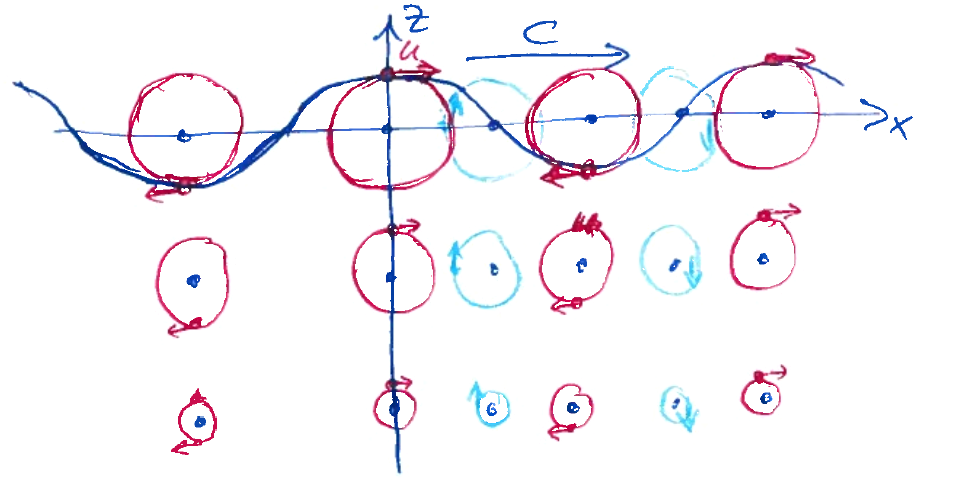
\includegraphics[width=.8\textwidth]{week6/surface-circle}\\
    \caption{}
    \label{fig:surface-circle}
\end{figure}

So far we have discussed a pure wave, which is characterized by the wave number $k$ and which travels with $c=\sqrt{\frac{g}{k}}=\sqrt{\frac{g\lambda}{2\pi}}$. The most general solution describing the spatio-temporal dynamics of the water surface is obtained by a superposition of different pure waves:
\begin{align}
\begin{split}
\Phi(x,z,t) &= \int_0^kdk\left[A(k)e^{i(kx+\omega t)}+B(k)e^{-i(kx+\omega t)}\right. \\
&\hspace{5mm}+\left.C(k)e^{i(kx-\omega t)}+D(k)e^{-i(kx-\omega t)}\right]
\end{split}
\end{align}

\begin{framed}
\textbf{Remark:} perturbation of a flat surface

A wave generated by this disturbance contains several different wave numbers $k$. Initial wane form is not stable; it decays since different $k$ components propagate with different phase velocities.
\end{framed}

\begin{framed}
\textbf{Remark:} small-amplitude surface waves at a finite depth ($d<\infty$)

\begin{align}
c &= \sqrt{\frac{g}{k}\tanh(kd)}\\
&= \sqrt{\frac{g\lambda}{2\pi}\tanh\left(2\pi\frac{d}{\lambda}\right)}
\end{align}

\begin{align}
d\gg\lambda&: \tanh(x\gg1)=0  \Rightarrow c=\sqrt{\frac{g\lambda}{2\pi}}\\
d\ll\lambda&: \tanh(x\ll1)=0 \Rightarrow c=\sqrt{gd}
\end{align}
\end{framed}

\textbf{More surface waves:}

\begin{itemize}
\item non-linear waves ($\lambda\gg d$): solitons
\item monster waves
\item wind-wave interaction
\item wave energy
\end{itemize}